\documentclass[12pt,a4paper]{article}
\usepackage[spanish]{babel}
\usepackage[utf8]{inputenc}

\usepackage[right=2cm,left=3cm,top=2cm,bottom=2cm,headsep=0cm,footskip=0.5cm]{geometry}
\usepackage{graphicx,subfigure}
\usepackage{amsmath}
\usepackage{underscore}

\graphicspath{ {img/} }

\title{\textbf{Análisis de \textit{El perro del hortelano}}}
\author{Alberto Navalón Lillo}

\begin{document}

\maketitle
\tableofcontents

\section{Introducción}

\textit{El perro del hortelano} es una obra teatral escrita por el dramaturgo español Lope de Vega y publicada en el año 1618, por lo que entra en el periodo correspondiente al Barroco. El período Barroco, que abarca todo el siglo XVII y principios del XVIII, fue originado por una nueva forma de concebir el arte, que recibe el mismo nombre (\textit{estilo barroco}), la cual, en términos generales, es la opuesta a la forma de concebir el arte en el período renacentista.\\

En este caso, en vez de englobar las características generales del Barroco, vamos a centrarnos en las del teatro de dicho período. En España, Lope de Vega fue uno de los autores con más influencia del Barroco, si no el que más. A él fueron contemporáneos otros autores de renombre como Tirso de Molina, Calderón de la Barca o Francisco de Rojas Zorrilla, junto a muchos otros. Dada su gran y notoria influencia, fue él mismo, con sus obras, quien estableció gran parte de las características del teatro barroco, por lo que estas se encuentran en sus obras claramente y en completa integridad.\\

A causa de esta concentración de dramaturgos en torno a este período, la cantidad y la calidad de obras teatrales, bien fuese teatro \textbf{religioso} (autos sacramentales), teatro \textbf{cortesano} o teatro \textbf{popular}, fue en aumento, lo que también hizo crecer el interés de las clases populares por el teatro, ya que era una forma atractiva de entretenerse.

\section{Características del teatro barroco en la obra}

Como ha sido mencionado anteriormente, en la introducción, Lope de Vega fue uno de los autores más importantes y representativos de la literatura barroca en general, por lo que tuvo una gran influencia en la misma. Y es por ello, que la inmensa mayoría de las obras de Lope contienen un gran número de características de la literatura barroca, dado que muchas de ellas se definieron posteriormente a partir de estas obras.

\subsection{La renovación del teatro por Lope de Vega}

En su \textit{Arte nuevo de hacer comedias}, Lope explica su nueva fórmula teatral, ajustada a los gustos del espectador de los corrales de comedias. En esta fórmula se basaron muchos dramaturgos posteriores para escribir sus obras. De entre los distintos elementos de esta fórmula, destacan por su aparición evidente en \textit{El perro del hortelano} tres de ellas.\\

En primer lugar, destaca la \textbf{ruptura} de las denominadas \textbf{tres unidades} (una acción, un emplazamiento, un día). Lope rompe con este convenio y añade complejidad a sus obras mediante la adición de acciones paralelas a la acción principal. En este caso, estas acciones paralelas serían, por ejemplo, las intenciones amorosas del resto de personajes (Marcela y Fabio, y el marqués Ricardo, el conde Federico y la condesa), es decir, los otros lados del triángulo amoroso, aparte del de Teodoro y la condesa Diana. Además, periódicamente se realizan saltos en el espacio y en el tiempo a lo largo de la obra, que se desarrolla fundamentalmente en el palacio de la condesa Diana, aunque la acción también se desplaza a la taberna de Nápoles y al palacio del conde Ludovico, en adición a desarrollarse a lo largo de varios días.\\

Para llevar a cabo esta variación espaciotemporal, la acción principal se desarrolla en \textbf{tres actos}, al igual que muchas otras obras de Lope, que, en términos aproximados, el primero, el segundo y el tercero corresponden con la introducción, el desarrollo y el desenlace de la obra, respectivamente.\\

Finalmente, en esta obra encontramos representados dos de los temas más representativos de la obra teatral de Lope: el \textbf{amor} y el \textbf{honor}. A pesar de que el amor está muy presente en esta obra (es el tema principal), en el triángulo amoroso que ocupa la acción principal (las intenciones amorosas de la condesa Diana y su secretario Teodoro), al igual que en la mayoría de acciones secundarias; el honor también ocupa una posición importante en la obra, dado que la condesa Diana no quiere perder su honor casándose con alguien de condición social inferior, Teodoro, a quien realmente ella ama. En adición a estos dos temas, también están presentes los celos, de ahí el título de esta comedia, que proviene del refrán «el perro del hortelano, que ni come ni deja comer». El título se analizará en más profundidad en a continuación.

\subsection{Los temas del teatro lopesco a partir del título}

El título de esta obra, como ya se ha mencionado anteriormente, proviene del refrán «el perro del hortelano, que ni come ni deja comer», el cual implica una reprensión a quien no disfruta de algo y además impide que otros lo hagan. Podemos dividir la segunda parte de este refrán en bloques:\\

\begin{figure}[h]
	\centering
	\subfigure[Fig. A: temas presentes en el refrán del perro del hortelano.]{\label{fig:a}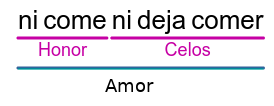
\includegraphics{refran}}
\end{figure}

De esta forma podemos observar cómo los tres temas que se desarrollan en la obra aparecen en el refrán en el cual se basa el título. A continuación se dará una explicación de cada uno de estos tres temas, y una justificación. Antes de ello, cabe mencionar que los tres temas, en el caso del refrán, corresponden a la condesa Diana, ya que es a ella a quién se asocia una similitud con el perro del hortelano.

\begin{itemize}
	\item El \textbf{honor} (\textit{ni come}): Diana tiene miedo de expresar públicamente su amor por Teodoro (\textit{comer}), dado que se arriesgaría a perder su honor, al ser Teodoro de condición social inferior.
	\item Los \textbf{celos} (\textit{ni deja comer}): al igual que ella no puede ``comer'', tampoco quiere que Teodoro ``coma'', es decir, que a pesar de que no tiene el valor para arriesgar su honor, tampoco quiere que Teodoro ame a otra mujer, ni que otra mujer ame a Teodoro, porque lo quiere para ella.
	\item El \textbf{amor} (\textit{ni come ni deja comer}): engloba todo el grupo, al igual que engloba toda la obra, al ser este el tema principal.
\end{itemize}

\section{Relación con el contexto histórico}

En esta obra no se puede observar muchas relaciones con el contexto histórico del momento (inicios del siglo XVII), por el hecho de que, a pesar de ese incremento de la complejidad y ese dinamismo espaciotemporal mencionado anteriormente, las acciones, tanto la principal como las paralelas a esta se desarrollan en espacios reducidos, y no encontramos muchas clases de personajes.\\

No obstante, podemos encontrar referencias al contexto social de la época, ya que en la obra encontramos, esencialmente, dos tipos de personajes: \textbf{nobles} (Diana, Ludovico, Ricardo, Federico...) y \textbf{criados} o \textbf{sirvientes} (Teodoro, Tristán, Marcela, Anarda, Dorotea, Fabio, Celio...), en definitiva, estos últimos de condición social inferior a los nobles. Esto hace referencia a la segregación estamental de la sociedad, que aún se mantenía al igual que en el medievo, con la única diferencia de que se había añadido la clase de la burguesía.\\

También hallamos referencias al contexto histórico del Imperio Español, que por este tiempo todavía estaba en buena forma, dado que la acción se desarrolla en Nápoles, que a principios del siglo XVII todavía formaba parte del reino de Felipe IV. Podemos deducir el tiempo externo de la obra mediante dos factores: la fecha de publicación (1618) y que Nápoles aún formaba parte del Imperio Español, por tanto, la fecha debía ser anterior a finales de la década de 1640, cuando se inicia una serie de sublevaciones internas que llevan a la pérdida de este territorio. Es también en esta década, con otros incidentes y conflictos, como la guerra de separación de Portugal, la rebelión de Cataluña o la conspiración de Andalucía, cuando la política española se inestabiliza, y es esta inestabilidad la que comienza el período que recibe el nombre de \textit{Decadencia española}, que lleva, varias décadas después, a perder territorios en América, así como otros territorios de ultramar. Al igual que a la pérdida de territorios, la inestabilidad política también lleva a una crisis social que se extiende hacia finales del siglo XVII.

\end{document}